%Empieza configuracion de capitulo
\setstretch{1.0}
\titleformat{\chapter}[block]{\Large\bfseries}{CAP'ITULO \Huge\thechapter\vspace{25 pt}}{0 pt}{\\\fontsize{26}{36}\selectfont}
\titlespacing{\chapter}{0 pt}{30 pt}{50 pt}[0 pt]
\titleformat{\section}{\Large\bfseries}{\thesection}{0 pt}{\hspace{30 pt}}
\titleformat{\subsection}{\large\bfseries}{\thesubsection}{0 pt}{\hspace{30 pt}}
\pagestyle{fancy}
\fancyhead[LO,LE]{\footnotesize\emph{\leftmark}}
\fancyhead[RO,RE]{\thepage}
\fancyfoot[CO,CE]{}
%Termina configuracion de capitulo

\chapter{Resultados} %Cambia al nombre de tu capitulo
\setstretch{1.5} %Regresa el interlineado a 1.5

\normalsize
\noindent
En el presente cap'itulo se describir'an los resultados de los experimentos realizados con los \emph{Observation Files}, la base de datos, y el ambiente en el cual fueron desarrollados.\\

\section{Descarga de archivos}
\noindent
Esta secci'on resume la distribuci'on de los diferentes tipos de archivos descargados a trav'es del software \emph{BNC-Ntrip Client}.

\begin{table}[H]
\begin{center}
\scalebox{0.9}{	
\begin{tabular}{| l || l | }
\hline
\textbf{Tipo de archivos} & \textbf{Tama'no(MB)} \\ \hline \hline
\emph{Observation Files} & 80,900 \\ \hline
\emph{Ephemerides Files} & 105 \\ \hline
\emph{Raw Data} & 14,500 \\ \hline
\emph{Log Files} & 4.25 \\ \hline
\end{tabular}}
\end{center}
\caption{Distribuci'on de los archivos descargados }
\end{table}

Tama'no total de los archivos descargados: 95.5 GB.\\

La siguiente tabla nos muestra la distribuci'on de los \emph{Observation Files}, entre los archivos correctos o legibles y los corruptos o ilegibles, ya sea por problemas de la red o de comunicaci'on entre el cliente y los \emph{broadcasters} o fallas el'ectricas del lado del cliente.

\begin{table}[H]
\begin{center}
\scalebox{0.9}{	
\begin{tabular}{| l || l | l |}
\hline
\textbf{Item} & \textbf{Cantidad} & \textbf{Porcentaje} \\ \hline \hline
Total de archivos & 40,792 & 100 \\ \hline
Total de archivos correctos & 40,775 & 99.96 \\ \hline
Total de archivos corruptos & 17 & 0.04 \\ \hline
\end{tabular}}
\end{center}
\caption{Distribuci'on de los \emph{Observation Files} }
\end{table}

Como resultado obtuvimos que menos del 1\% fueron archivos totalmente ilegibles y por ende no hicieron parte de los experimentos hechos.\\

La presente gr'afica nos muestra la tendencia de descarga a lo largo de 4 meses.

\begin{figure}[H]
\centering
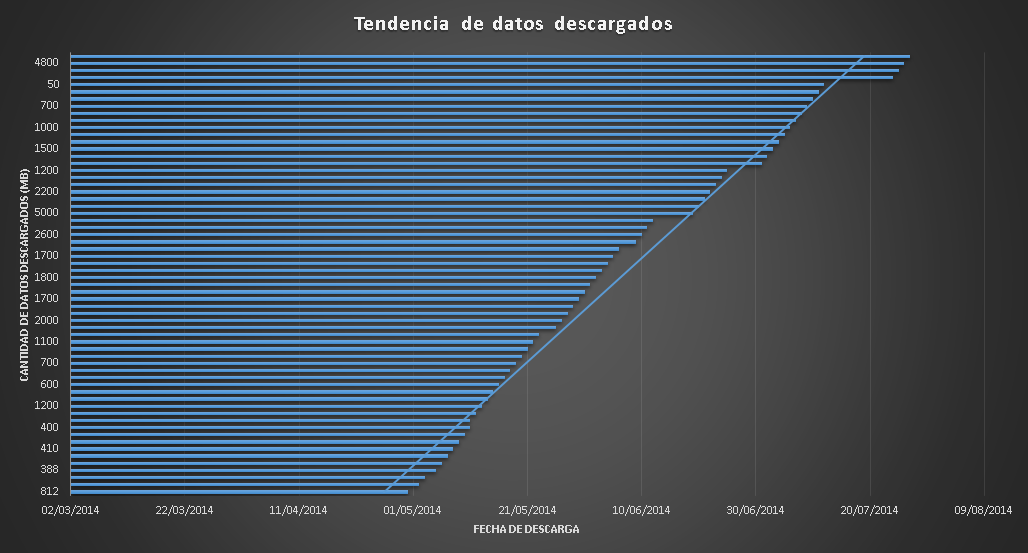
\includegraphics[width=0.95\textwidth]{images/Tendencia_Datos_Descargados}
\caption{Tendencia de archivos descargados}
\label{fig:6.1}
\end{figure}

La figura 6.1 nos indica que al cabo del tiempo de descarga de datos definido, se necesit'o mayor tiempo de ejecuci'on de la aplicaci'on para obtener una mayor cantidad de datos para ser procesados, con el objetivo de llegar a una muestra considerable de datos en un menor tiempo.

\section{Resultados de las pruebas}
\noindent
En la presente secci'on se presentan los resultados obtenidos en las diferentes pruebas. Se describen los resultados del tiempo de ejecuci'on como tambi'en se ilustran con gr'aficas diferentes m'etricas de rendimiento, como lo son el uso del CPU y de la memoria. \\

Para determinar y monitorear las diferentes m'etricas se hizo de la herramienta \emph{VisualVM}, la cual es una herramienta que muestra informaci'on detallada de las aplicaciones \emph{Java} que se ejecutan en la \emph{Java Virtual Machine (JVM)}. \\

\subsection{Base de datos}
\noindent
La presente tabla muestra la cantidad de registros insertados en la base de datos, en las tablas METADATA, OBSERVATION\_DATA, y LLI, pertenecientes al meta-modelo.

\begin{table}[H]
\begin{center}
\scalebox{0.9}{	
\begin{tabular}{| l || l | }
\hline
\textbf{Tabla} & \textbf{Cantidad de registros} \\ \hline \hline
\emph{METADATA} & 40,775 \\ \hline
\emph{OBSERVATION\_DATA} & 34'200,319 \\ \hline
\emph{LLI} & 12'089,001 \\ \hline
\end{tabular}}
\end{center}
\caption{Distribuci'on de registros en las tablas del meta-modelo}
\end{table}

Dentro de esta cantidad de registros no se encontr'o ninguna falla entre las \emph{epoch dates}. Esto quiere decir que durante el tiempo de toma de las m'etricas u observaciones por parte de los \emph{GNSS} no se gener'o ning'un evento que alterara el valor observado. \\

En la siguiente tabla se muestra la cantidad de registros referentes al \emph{Loss of Lock Indicator} con un posible deslizamiento de ciclo en los tipos de observaciones L1 y L2, almacenados en la tabla LLI.

\begin{table}[H]
\begin{center}
\scalebox{0.9}{	
\begin{tabular}{| l || l | }
\hline
\textbf{Tipo de observaci'on} & \textbf{Cantidad de registros} \\ \hline \hline
L1 & 2'517,286 \\ \hline
L2 & 1'431,922 \\ \hline
\end{tabular}}
\end{center}
\caption{Cantidad de registros con posible deslizamiento de ciclo, L1 y L2}
\end{table}

A continuaci'on se muestran las frecuencias y la cantidad de posibles deslizamiento de ciclos referentes al \emph{Loss of Lock Indicator} de los tipos de observaciones L1 y L2 por d'ia, es decir, durante el tiempo de obtenci'on de los datos.\\

\begin{figure}[H]
\centering
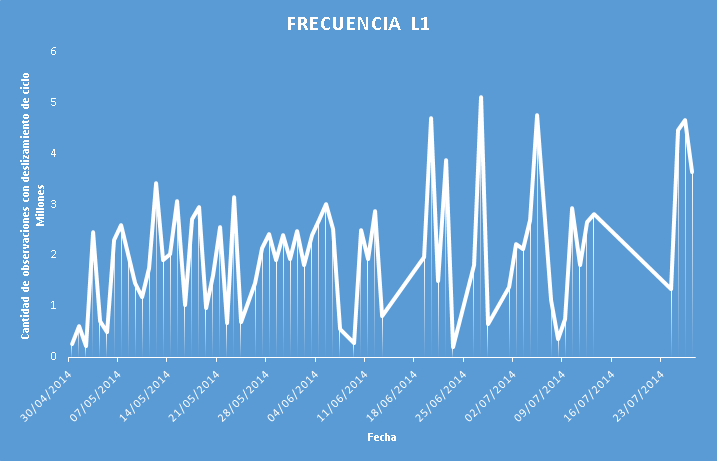
\includegraphics[width=0.95\textwidth]{images/Frecuency_L1}
\caption{Frecuencia L1}
\label{fig:6.2}
\end{figure}

\begin{figure}[H]
\centering
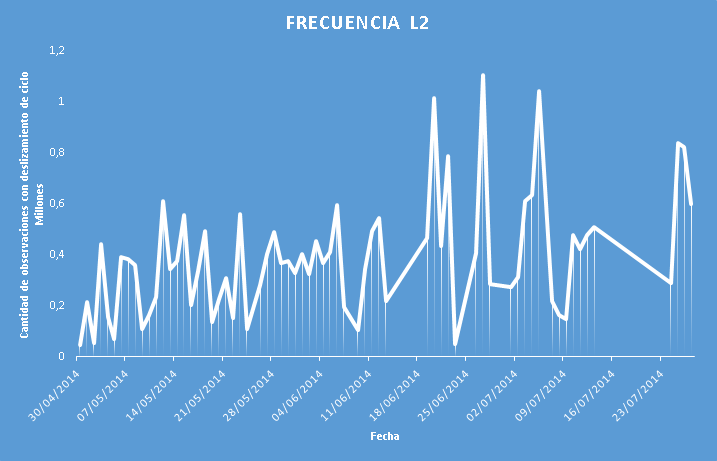
\includegraphics[width=0.95\textwidth]{images/Frecuency_L2}
\caption{Frecuencia L2}
\label{fig:6.3}
\end{figure}

\begin{figure}[H]
\centering
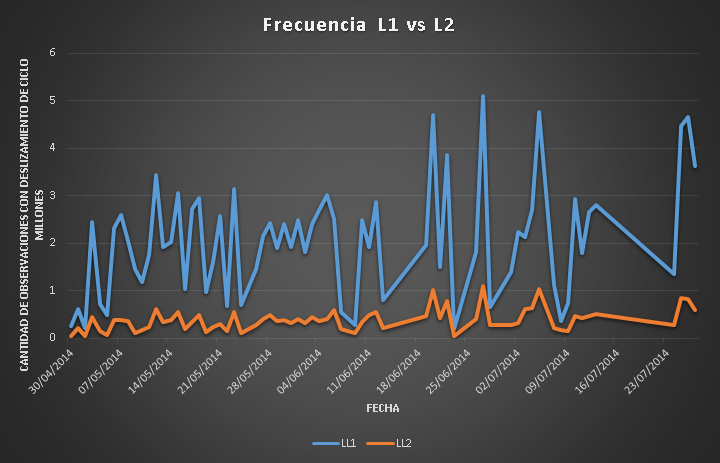
\includegraphics[width=0.95\textwidth]{images/Frecuency_L1_L2}
\caption{Frecuencia L1 y L2}
\label{fig:6.4}
\end{figure}

La cantidad m'axima de observaciones con posible deslizamiento de ciclo para L1 fue de 5.107.444 y de 1.105.203 para L2. Mientras que los valores m'inimos fueron 199.511 y 46.604 para L1 y L2 respectivamente. \\

Con esta informaci'on interpretamos que una de las anomal'ias m'as comunes en los tipos de observaciones L1 y L2 es el deslizamiento de ciclo, igualmente esta no representa como tal una falla del valor observado, solo nos indica que se debe realizar un proceso de correcci'on para hallar el valor correcto observado. Estas correcciones se realizan a trav'es de diferentes m'etodos, los cuales no hacen parte de esta investigaci'on. \\

Las figuras 6.5, 6.6 y 6.7 nos resumen por cada uno de los meses, las frecuencias del \emph{Loss of Lock Indicator} para L1 y L2. \\

\begin{figure}[H]
\centering
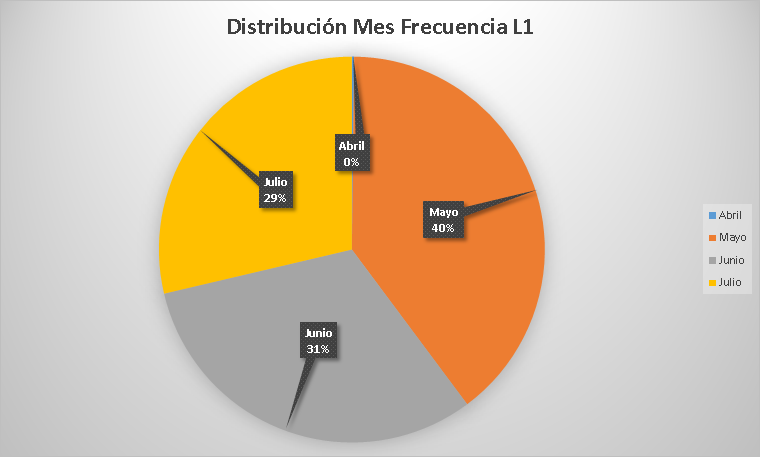
\includegraphics[width=0.95\textwidth]{images/Frecuency_Month_L1}
\caption{Frecuencia mes, L1}
\label{fig:6.5}
\end{figure}

\begin{figure}[H]
\centering
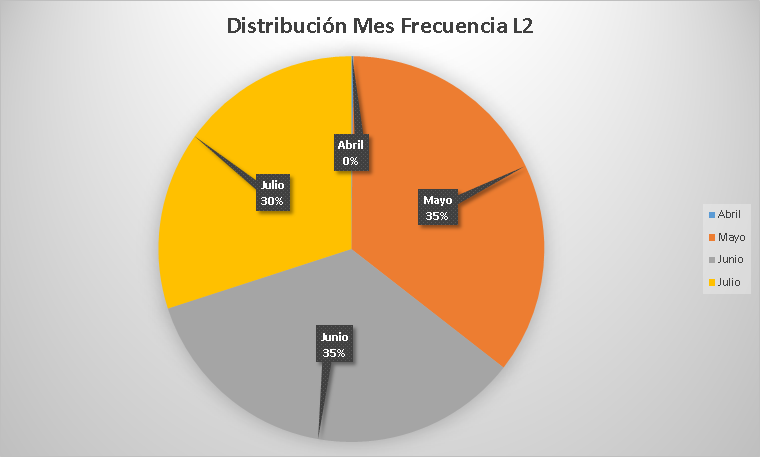
\includegraphics[width=0.95\textwidth]{images/Frecuency_Month_L2}
\caption{Frecuencia mes, L2}
\label{fig:6.6}
\end{figure}

\begin{figure}[H]
\centering
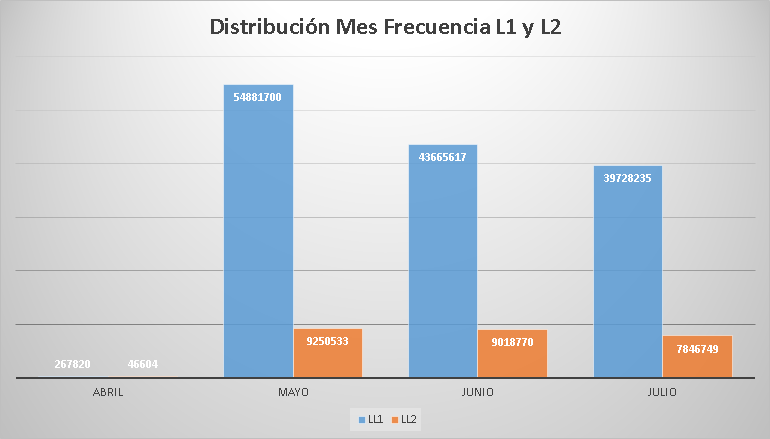
\includegraphics[width=0.95\textwidth]{images/Frecuency_Month_L1_L2}
\caption{Frecuencia mes, L1 y L2}
\label{fig:6.7}
\end{figure}

\subsection{Modo secuencial}
\noindent
En la siguiente tabla se muestran los resultados obtenidos de las ejecuciones en modo serial.

\begin{table}[H]
\begin{center}
\scalebox{0.9}{	
\begin{tabular}{| c || c | c | c | }
\hline
\textbf{N'umero de} & \textbf{Tiempo de} & \textbf{Tiempo de} & \textbf{Tiempo de}\\ 
\textbf{ejecuci'on} & \textbf{ejecuci'on} & \textbf{ejecuci'on} & \textbf{ejecuci'on}\\ 
& \textbf{(segundos)} & \textbf{(minutos)} & \textbf{(horas)} \\ \hline \hline
1 & 5962.77 & 99.38	& 1.66 \\ \hline
2 & 6294.33	& 104.91 & 1.75 \\ \hline
3 & 5949.65	& 99.16	& 1.65 \\ \hline
\textbf{Promedio} & \textbf{6068.92} & \textbf{101.15} & \textbf{1.69} \\ \hline
\end{tabular}}
\end{center}
\caption{Resultados en modo secuencial}
\end{table}

En las figuras 6.8, 6.9, 6.10, 6.11 y 6.12, se evidencia el rendimiento en t'erminos de uso del CPU del \emph{workstation}, la memoria RAM utilizada por la \emph{Java Virtual Machine (JVM)},  el tiempo de ejecuci'on del hilo principal, la cantidad de hilos y \emph{demons} con su rango (en tiempo) de ``vida''.

\begin{figure}[H]
\centering
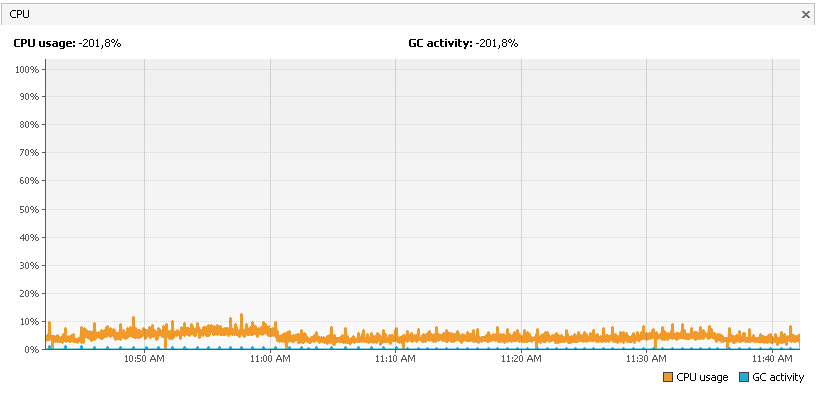
\includegraphics[width=0.95\textwidth]{images/Performance_CPU_1_Threads}
\caption{\emph{Performance CPU}, con un hilo principal}
\label{fig:6.8}
\end{figure}

\begin{figure}[H]
\centering
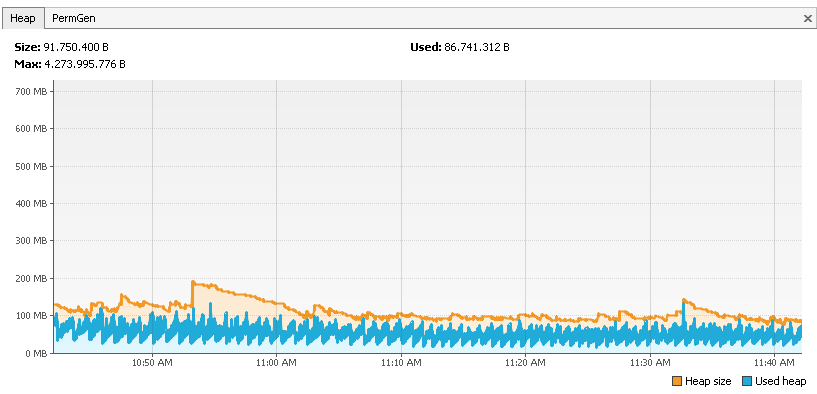
\includegraphics[width=0.95\textwidth]{images/Performance_HEAP_1_Threads}
\caption{\emph{Performance - Heap memory}, con un hilo principal}
\label{fig:6.9}
\end{figure}

\begin{figure}[H]
\centering
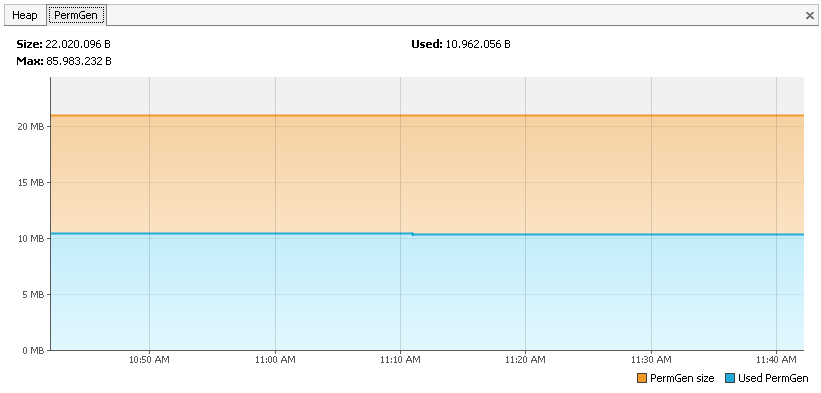
\includegraphics[width=0.95\textwidth]{images/Performance_PERM_1_Threads}
\caption{\emph{Performance - Permanent Generation heap}, con un hilo principal}
\label{fig:6.10}
\end{figure}

\begin{figure}[H]
\centering
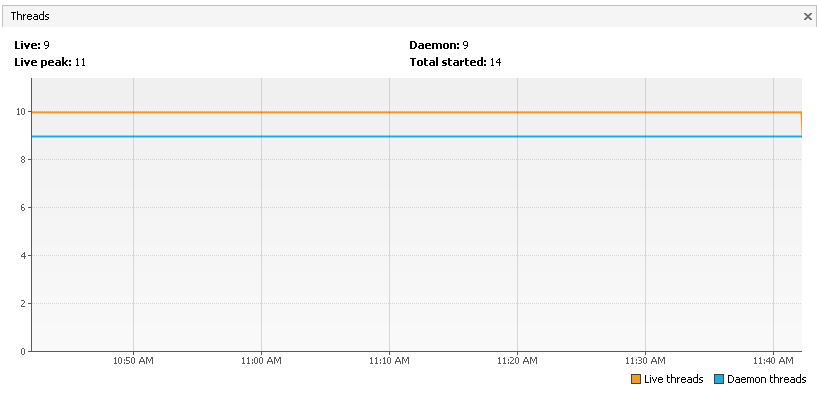
\includegraphics[width=0.95\textwidth]{images/Performance_LIVE_1_Threads}
\caption{\emph{Performance - Live demons and threads}, con un hilo principal}
\label{fig:6.11}
\end{figure}

\begin{figure}[H]
\centering
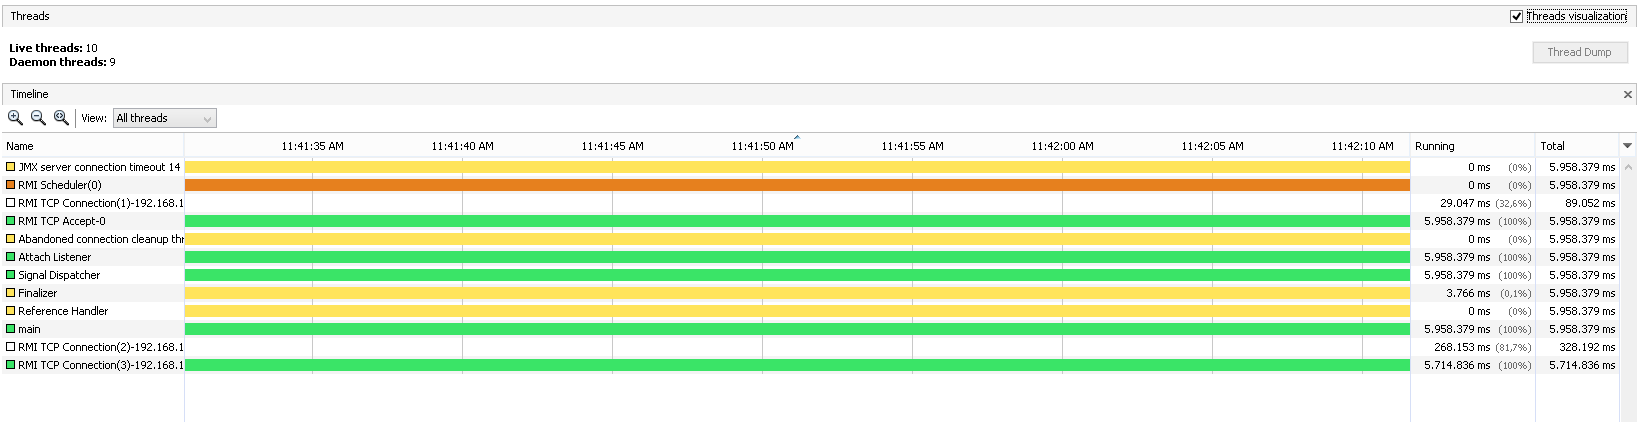
\includegraphics[width=0.95\textwidth]{images/Running_Time_1_Threads}
\caption{\emph{Thread timeline}, con un hilo principal}
\label{fig:6.12}
\end{figure}

\subsection{Modo paralelo, 8 \emph{Threads}}
\noindent
La configuraci'on del \emph{pool} de conexiones usada fue: \\

\textbf{Tama'no inicial} = 16 conexiones. \\
\textbf{N'umero m'aximo de conexiones activas} = 14. \\
\textbf{N'umero m'aximo de \emph{prepared statements} activas} = 14. \\

En la siguiente tabla se muestran los resultados obtenidos de las ejecuciones en modo paralelo utilizando 8 hilos. \\

\begin{table}[H]
\begin{center}
\scalebox{0.9}{	
\begin{tabular}{| c || c | c | c | }
\hline
\textbf{N'umero de} & \textbf{Tiempo de} & \textbf{Tiempo de} & \textbf{Tiempo de}\\ 
\textbf{ejecuci'on} & \textbf{ejecuci'on} & \textbf{ejecuci'on} & \textbf{ejecuci'on}\\ 
& \textbf{(segundos)} & \textbf{(minutos)} & \textbf{(horas)} \\ \hline \hline
1 & 2797.30	& 46.62	& 0.78 \\ \hline
2 & 3045.28	& 50.75	& 0.85 \\ \hline
3 & 2859.42	& 47.66	& 0.79 \\ \hline
\textbf{Promedio} & \textbf{2900.67} & \textbf{48.34} & \textbf{0.81} \\ \hline
\end{tabular}}
\end{center}
\caption{Resultados en modo paralelo con 8 hilos}
\end{table}

\begin{figure}[H]
\centering
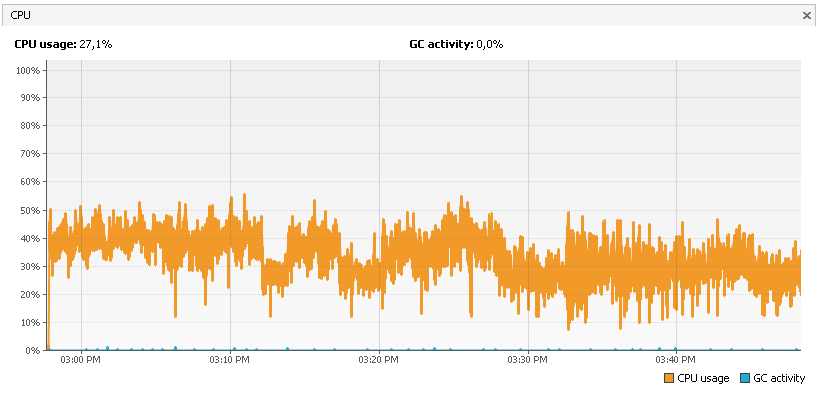
\includegraphics[width=0.95\textwidth]{images/Performance_CPU_8_Threads}
\caption{\emph{Performance CPU}, con 8 hilos}
\label{fig:6.13}
\end{figure}

\begin{figure}[H]
\centering
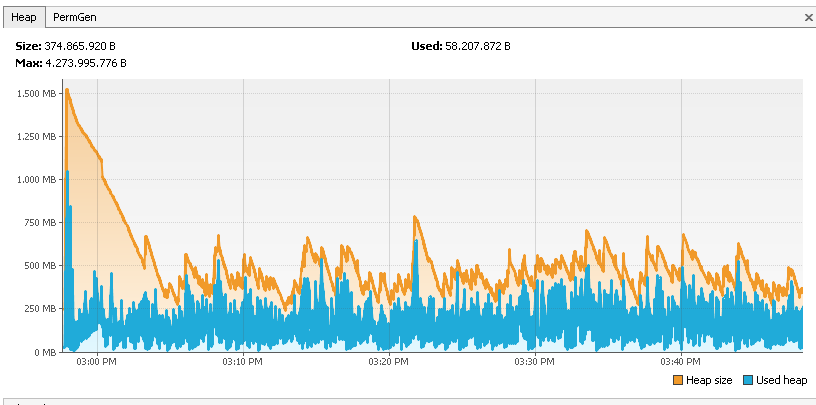
\includegraphics[width=0.95\textwidth]{images/Performance_HEAP_8_Threads}
\caption{\emph{Performance - Heap memory}, con 8 hilos}
\label{fig:6.14}
\end{figure}

\begin{figure}[H]
\centering
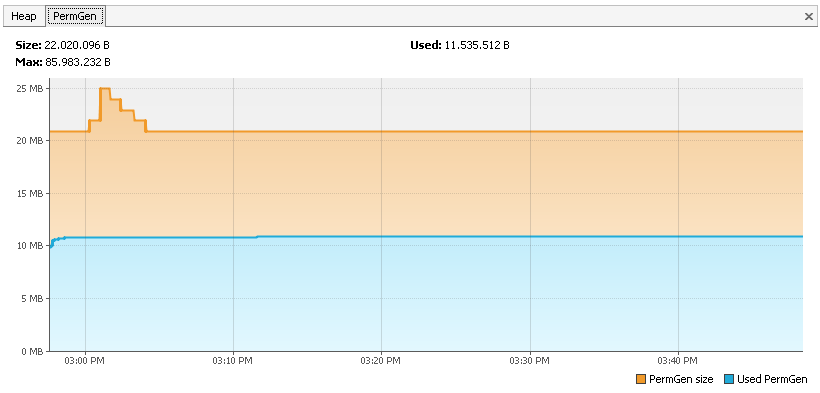
\includegraphics[width=0.95\textwidth]{images/Performance_PERM_8_Threads}
\caption{\emph{Performance - Permanent Generation heap}, con 8 hilos}
\label{fig:6.15}
\end{figure}

\begin{figure}[H]
\centering
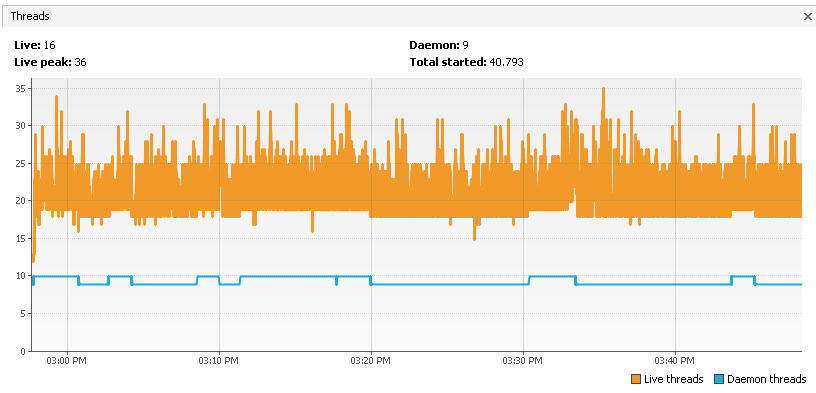
\includegraphics[width=0.95\textwidth]{images/Performance_LIVE_8_Threads}
\caption{\emph{Performance - Live demons and threads}, con 8 hilos}
\label{fig:6.16}
\end{figure}

\begin{figure}[H]
\centering
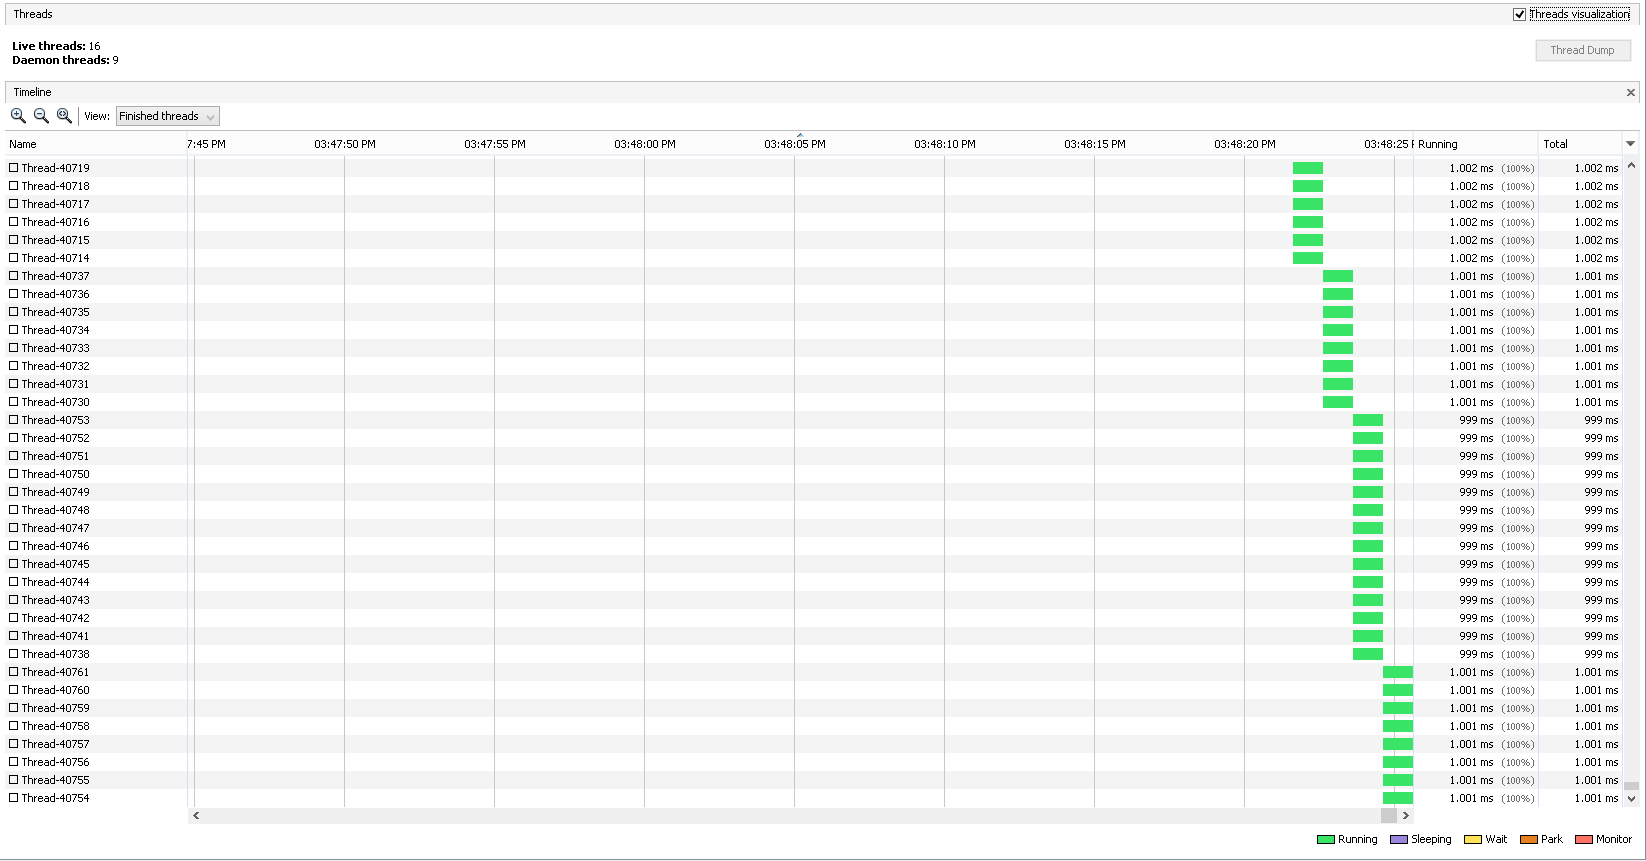
\includegraphics[width=0.95\textwidth]{images/Running_Time_8_Threads}
\caption{\emph{Thread timeline}, con 8 hilos}
\label{fig:6.17}
\end{figure}

\subsection{Modo paralelo, 10 \emph{Threads}}
\noindent
La configuraci'on del \emph{pool} de conexiones usada fue: \\

\textbf{Tama'no inicial} = 25 conexiones. \\
\textbf{N'umero m'aximo de conexiones activas} = 20. \\
\textbf{N'umero m'aximo de \emph{prepared statements} activas} = 20. \\

En la siguiente tabla se muestran los resultados obtenidos de las ejecuciones en modo paralelo utilizando 10 hilos. \\

\begin{table}[H]
\begin{center}
\scalebox{0.9}{	
\begin{tabular}{| c || c | c | c | }
\hline
\textbf{N'umero de} & \textbf{Tiempo de} & \textbf{Tiempo de} & \textbf{Tiempo de}\\ 
\textbf{ejecuci'on} & \textbf{ejecuci'on} & \textbf{ejecuci'on} & \textbf{ejecuci'on}\\ 
& \textbf{(segundos)} & \textbf{(minutos)} & \textbf{(horas)} \\ \hline \hline
1 & 2655.83	& 44.26	& 0.74 \\ \hline
2 & 2811.69	& 46.86	& 0.78 \\ \hline
3 & 2861.03	& 47.68	& 0.79 \\ \hline
\textbf{Promedio} & \textbf{2776.18} & \textbf{46.27} & \textbf{0.77} \\ \hline
\end{tabular}}
\end{center}
\caption{Resultados en modo paralelo con 10 hilos}
\end{table}

\begin{figure}[H]
\centering
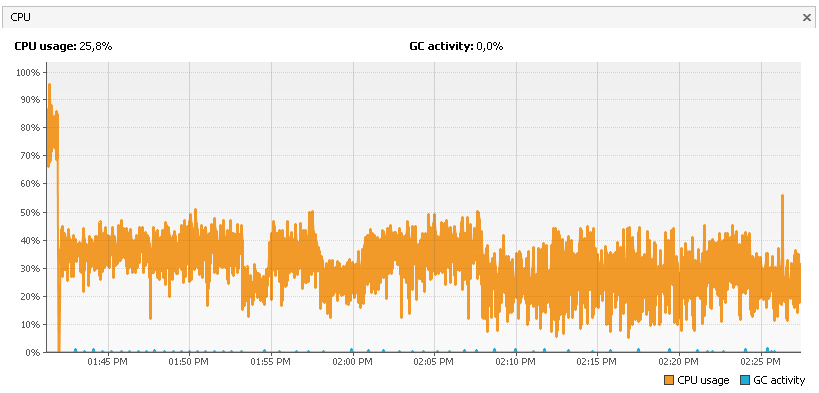
\includegraphics[width=0.95\textwidth]{images/Performance_CPU_10_Threads}
\caption{\emph{Performance CPU}, con 10 hilos}
\label{fig:6.18}
\end{figure}

\begin{figure}[H]
\centering
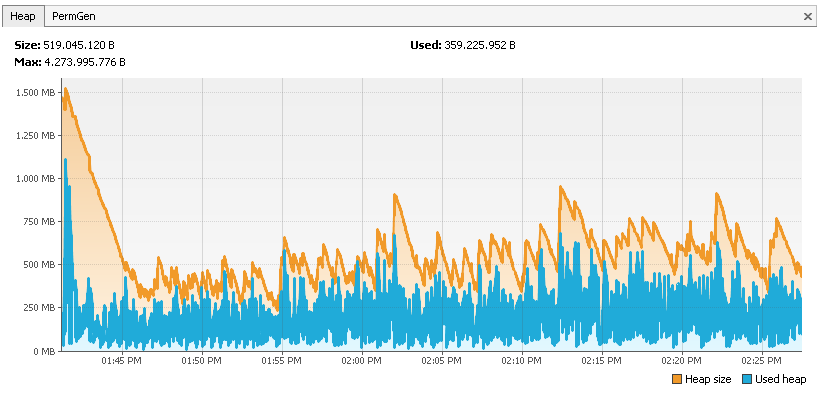
\includegraphics[width=0.95\textwidth]{images/Performance_HEAP_10_Threads}
\caption{\emph{Performance - Heap memory}, con 10 hilos}
\label{fig:6.19}
\end{figure}

\begin{figure}[H]
\centering
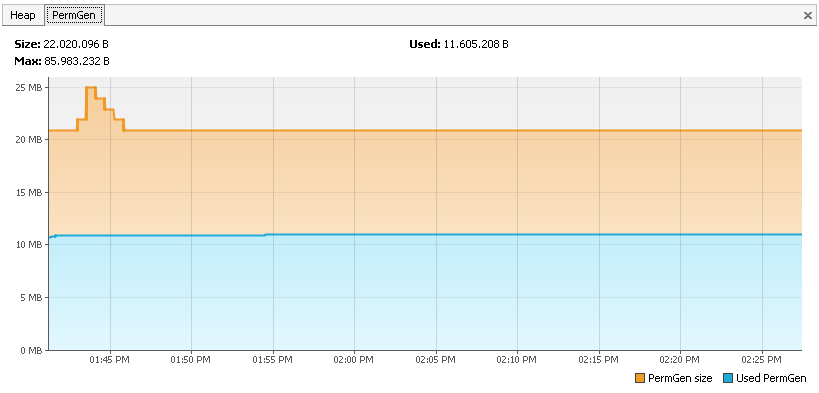
\includegraphics[width=0.95\textwidth]{images/Performance_PERM_10_Threads}
\caption{\emph{Performance - Permanent Generation heap}, con 10 hilos}
\label{fig:6.20}
\end{figure}

\begin{figure}[H]
\centering
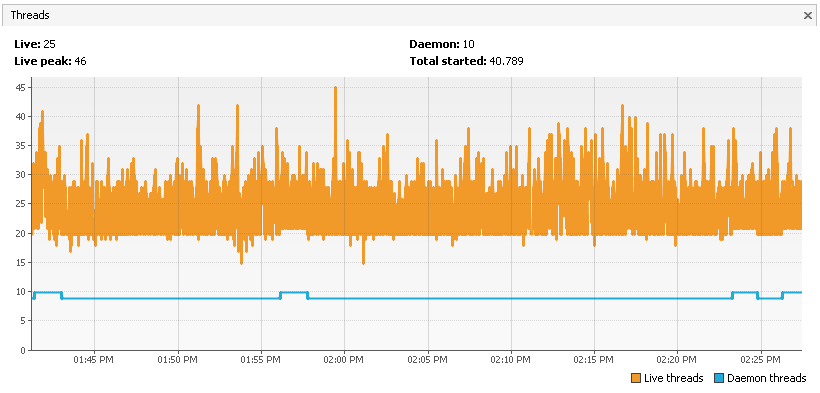
\includegraphics[width=0.95\textwidth]{images/Performance_LIVE_10_Threads}
\caption{\emph{Performance - Live demons and threads}, con 10 hilos}
\label{fig:6.21}
\end{figure}

\begin{figure}[H]
\centering
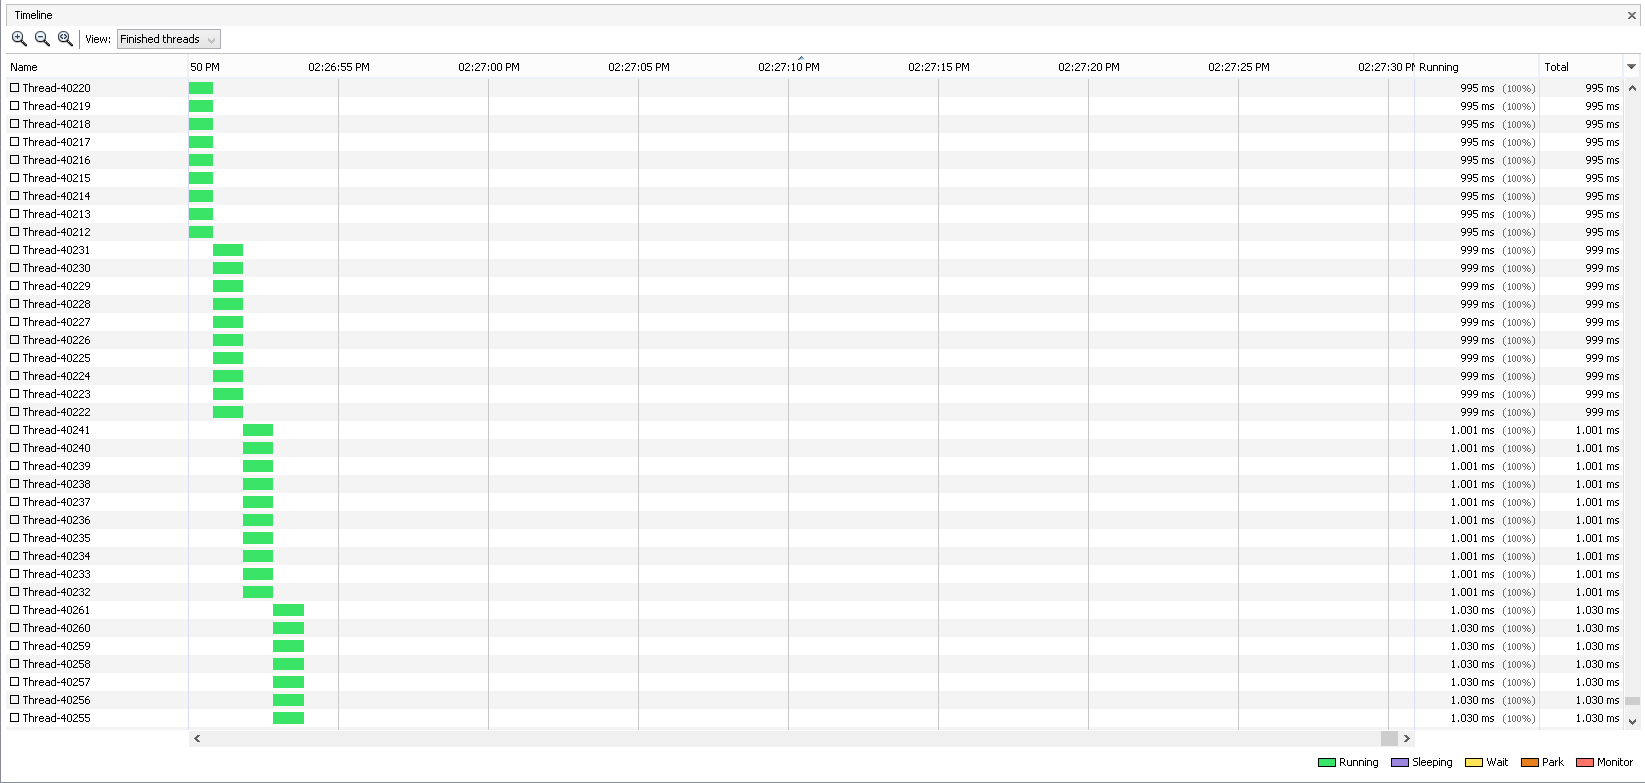
\includegraphics[width=0.95\textwidth]{images/Running_Time_10_Threads}
\caption{\emph{Thread timeline}, con 10 hilos}
\label{fig:6.22}
\end{figure}

\subsection{Modo paralelo, 16 \emph{Threads}}
\noindent
La configuraci'on del \emph{pool} de conexiones usada fue: \\

\textbf{Tama'no inicial} = 35 conexiones. \\
\textbf{N'umero m'aximo de conexiones activas} = 32. \\
\textbf{N'umero m'aximo de \emph{prepared statements} activas} = 32. \\

En la siguiente tabla se muestran los resultados obtenidos de las ejecuciones en modo paralelo utilizando 16 hilos. \\

\begin{table}[H]
\begin{center}
\scalebox{0.9}{	
\begin{tabular}{| c || c | c | c | }
\hline
\textbf{N'umero de} & \textbf{Tiempo de} & \textbf{Tiempo de} & \textbf{Tiempo de}\\ 
\textbf{ejecuci'on} & \textbf{ejecuci'on} & \textbf{ejecuci'on} & \textbf{ejecuci'on}\\ 
& \textbf{(segundos)} & \textbf{(minutos)} & \textbf{(horas)} \\ \hline \hline
1 & 3999.67	& 66.66	& 1.11 \\ \hline
2 & 4026.75	& 67.11	& 1.12 \\ \hline
3 & 4044.03	& 67.40	& 1.12 \\ \hline
\textbf{Promedio} & \textbf{4023.48} & \textbf{67.06} & \textbf{1.12} \\ \hline
\end{tabular}}
\end{center}
\caption{Resultados en modo paralelo con 16 hilos}
\end{table}

\begin{figure}[H]
\centering
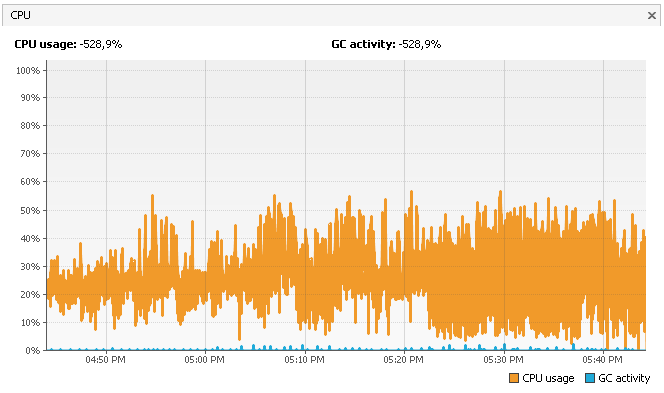
\includegraphics[width=0.95\textwidth]{images/Performance_CPU_16_Threads}
\caption{\emph{Performance CPU}, con 16 hilos}
\label{fig:6.23}
\end{figure}

\begin{figure}[H]
\centering
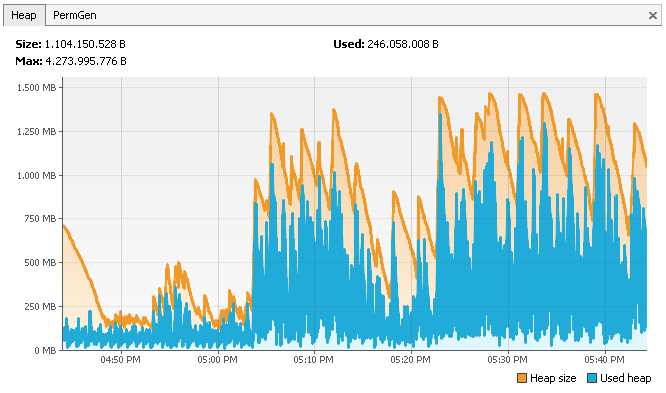
\includegraphics[width=0.95\textwidth]{images/Performance_HEAP_16_Threads}
\caption{\emph{Performance - Heap memory}, con 16 hilos}
\label{fig:6.24}
\end{figure}

\begin{figure}[H]
\centering
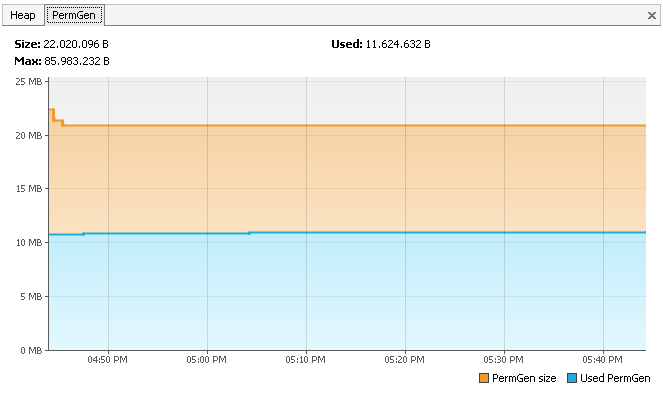
\includegraphics[width=0.95\textwidth]{images/Performance_PERM_16_Threads}
\caption{\emph{Performance - Permanent Generation heap}, con 16 hilos}
\label{fig:6.25}
\end{figure}

\begin{figure}[H]
\centering
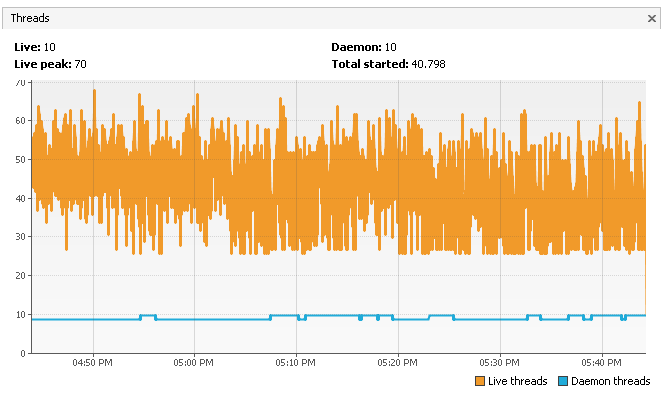
\includegraphics[width=0.95\textwidth]{images/Performance_LIVE_16_Threads}
\caption{\emph{Performance - Live demons and threads}, con 16 hilos}
\label{fig:6.26}
\end{figure}

\begin{figure}[H]
\centering
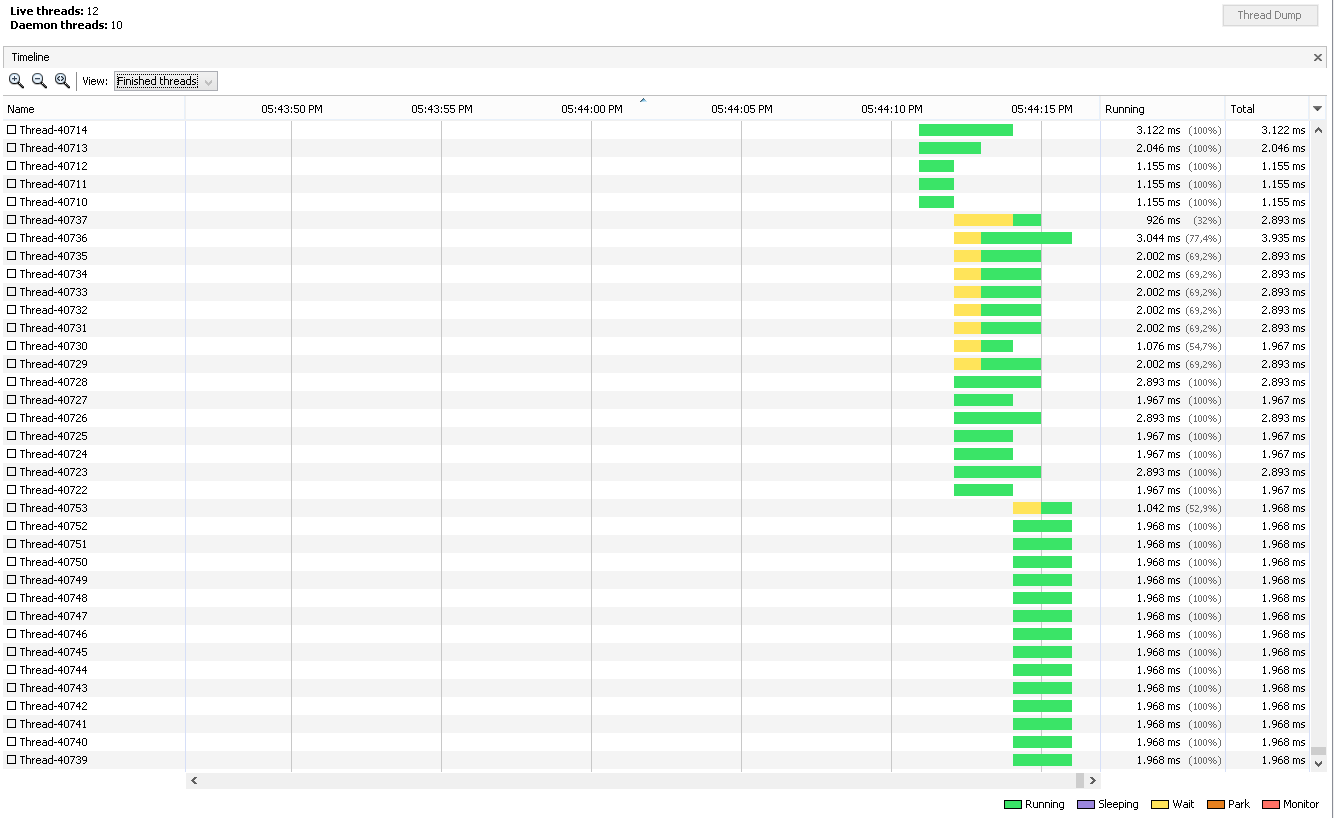
\includegraphics[width=0.95\textwidth]{images/Running_Time_16_Threads}
\caption{\emph{Thread timeline}, con 16 hilos}
\label{fig:6.27}
\end{figure}

\subsection{Modo paralelo, 32 \emph{Threads}}
\noindent
La configuraci'on del \emph{pool} de conexiones usada fue: \\

\textbf{Tama'no inicial} = 70 conexiones. \\
\textbf{N'umero m'aximo de conexiones activas} = 64. \\
\textbf{N'umero m'aximo de \emph{prepared statements} activas} = 64. \\

En la siguiente tabla se muestran los resultados obtenidos de las ejecuciones en modo paralelo utilizando 32 hilos. \\

\begin{table}[H]
\begin{center}
\scalebox{0.9}{	
\begin{tabular}{| c || c | c | c | }
\hline
\textbf{N'umero de} & \textbf{Tiempo de} & \textbf{Tiempo de} & \textbf{Tiempo de}\\ 
\textbf{ejecuci'on} & \textbf{ejecuci'on} & \textbf{ejecuci'on} & \textbf{ejecuci'on}\\ 
& \textbf{(segundos)} & \textbf{(minutos)} & \textbf{(horas)} \\ \hline \hline
1 & 28420.19 & 473.67 & 7.89 \\ \hline
2 & 28268.55 & 471.14 & 7.85 \\ \hline
3 & 28735.94 & 478.93 & 7.98 \\ \hline
\textbf{Promedio} & \textbf{28474.89} & \textbf{474.58} & \textbf{7.91} \\ \hline
\end{tabular}}
\end{center}
\caption{Resultados en modo paralelo con 32 hilos}
\end{table}

\begin{figure}[H]
\centering
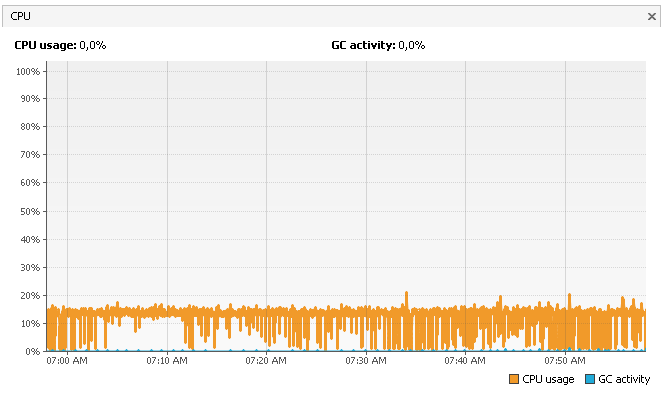
\includegraphics[width=0.95\textwidth]{images/Performance_CPU_32_Threads}
\caption{\emph{Performance CPU}, con 32 hilos}
\label{fig:6.28}
\end{figure}

\begin{figure}[H]
\centering
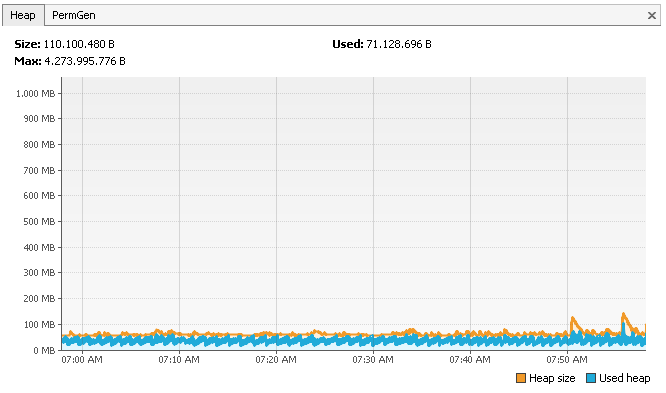
\includegraphics[width=0.95\textwidth]{images/Performance_HEAP_32_Threads}
\caption{\emph{Performance - Heap memory}, con 32 hilos}
\label{fig:6.29}
\end{figure}

\begin{figure}[H]
\centering
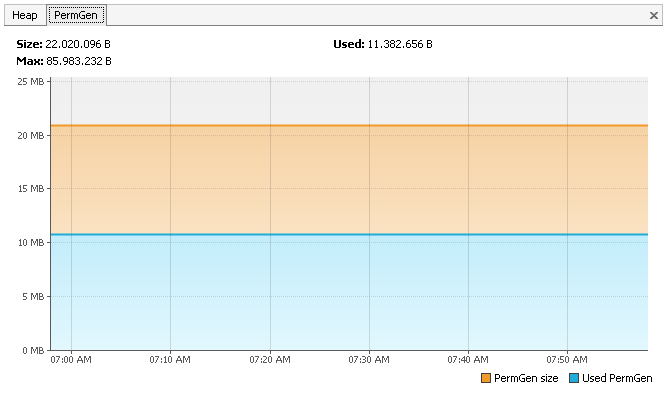
\includegraphics[width=0.95\textwidth]{images/Performance_PERM_32_Threads}
\caption{\emph{Performance - Permanent Generation heap}, con 32 hilos}
\label{fig:6.30}
\end{figure}

\begin{figure}[H]
\centering
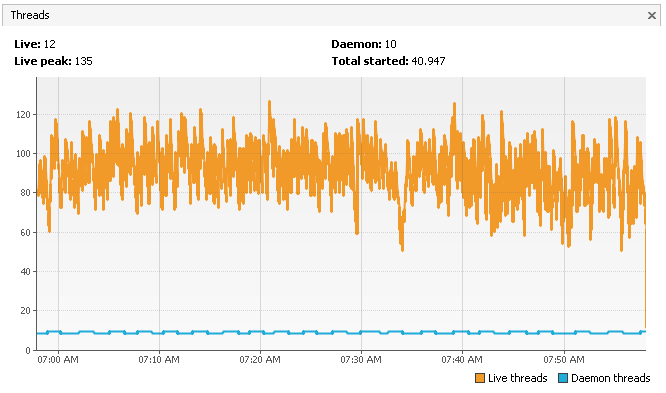
\includegraphics[width=0.95\textwidth]{images/Performance_LIVE_32_Threads}
\caption{\emph{Performance - Live demons and threads}, con 32 hilos}
\label{fig:6.31}
\end{figure}

\begin{figure}[H]
\centering
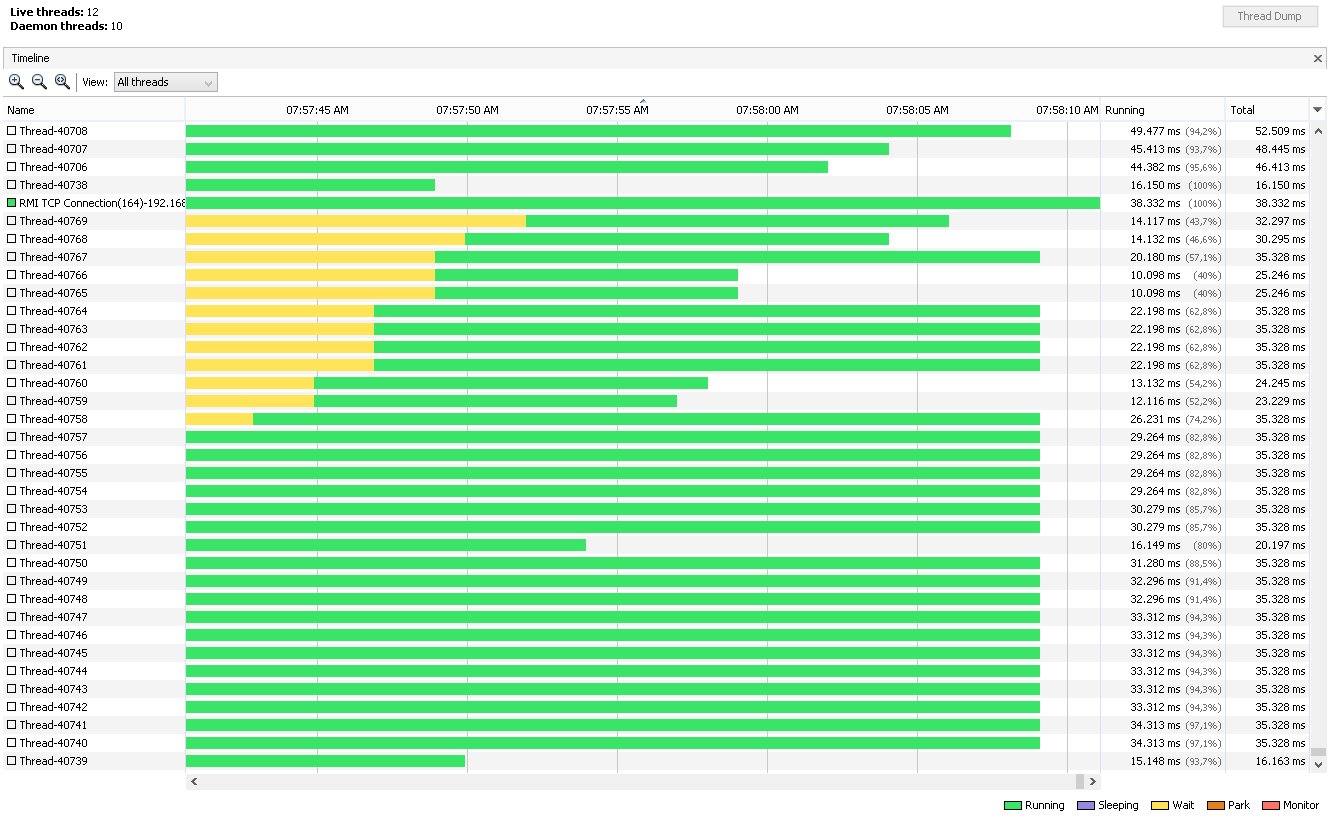
\includegraphics[width=0.95\textwidth]{images/Running_Time_32_Threads}
\caption{\emph{Thread timeline}, con 32 hilos}
\label{fig:6.32}
\end{figure}

\subsection{Modo paralelo, 50 \emph{Threads}}
\noindent
La configuraci'on del \emph{pool} de conexiones usada fue: \\

\textbf{Tama'no inicial} = 100 conexiones. \\
\textbf{N'umero m'aximo de conexiones activas} = 75. \\
\textbf{N'umero m'aximo de \emph{prepared statements} activas} = 75. \\

En la siguiente tabla se muestran los resultados obtenidos de las ejecuciones en modo paralelo utilizando 50 hilos. \\

\begin{table}[H]
\begin{center}
\scalebox{0.9}{	
\begin{tabular}{| c || c | c | c | }
\hline
\textbf{N'umero de} & \textbf{Tiempo de} & \textbf{Tiempo de} & \textbf{Tiempo de}\\ 
\textbf{ejecuci'on} & \textbf{ejecuci'on} & \textbf{ejecuci'on} & \textbf{ejecuci'on}\\ 
& \textbf{(segundos)} & \textbf{(minutos)} & \textbf{(horas)} \\ \hline \hline
1 & 30543.12 & 509.05 & 8.48 \\ \hline
2 & 31362.10 & 522.70 & 8.71 \\ \hline
3 & 32208.99 & 536.82 & 8.95 \\ \hline
\textbf{Promedio} & \textbf{31371.40} & \textbf{522.86} & \textbf{8.71} \\ \hline
\end{tabular}}
\end{center}
\caption{Resultados en modo paralelo con 50 hilos}
\end{table}

\begin{figure}[H]
\centering
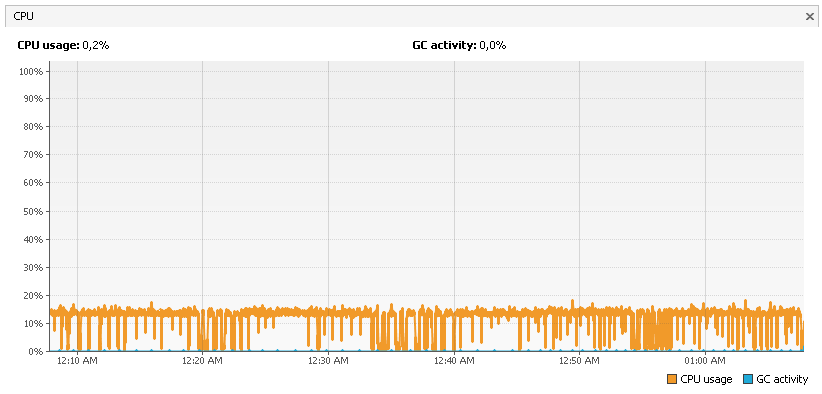
\includegraphics[width=0.95\textwidth]{images/Performance_CPU_50_Threads}
\caption{\emph{Performance CPU}, con 50 hilos}
\label{fig:6.33}
\end{figure}

\begin{figure}[H]
\centering
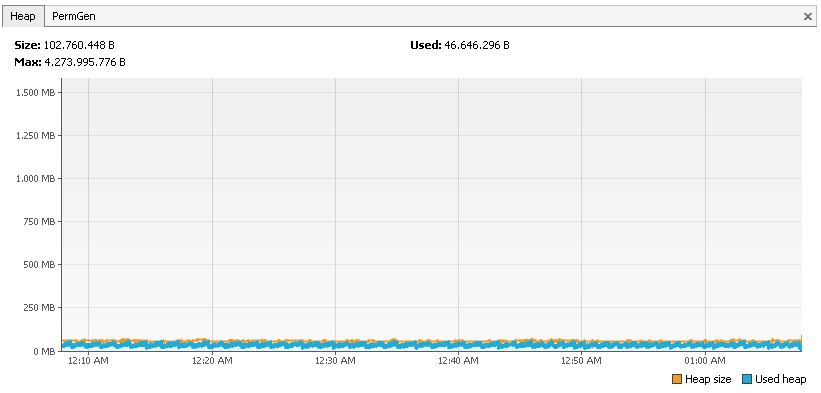
\includegraphics[width=0.95\textwidth]{images/Performance_HEAP_50_Threads}
\caption{\emph{Performance - Heap memory}, con 50 hilos}
\label{fig:6.34}
\end{figure}

\begin{figure}[H]
\centering
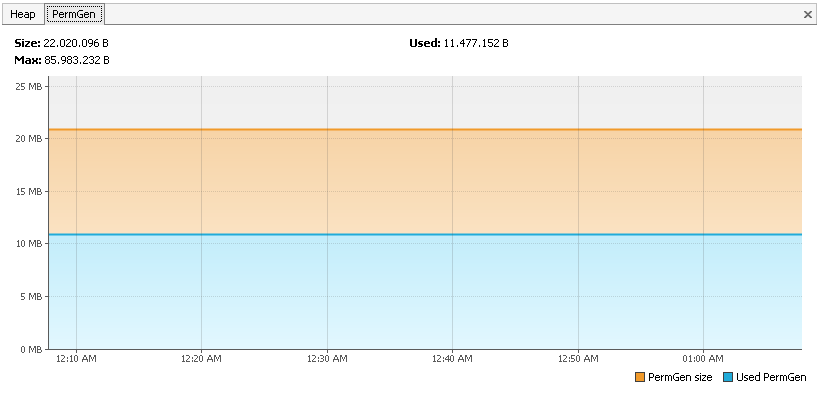
\includegraphics[width=0.95\textwidth]{images/Performance_PERM_50_Threads}
\caption{\emph{Performance - Permanent Generation heap}, con 50 hilos}
\label{fig:6.35}
\end{figure}

\begin{figure}[H]
\centering
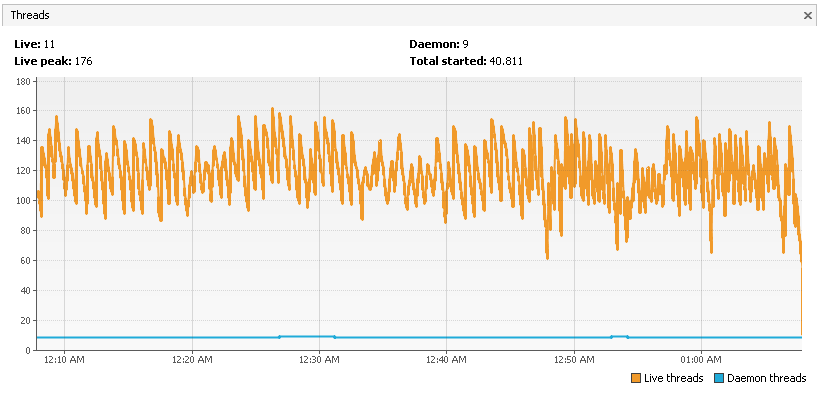
\includegraphics[width=0.95\textwidth]{images/Performance_LIVE_50_Threads}
\caption{\emph{Performance - Live demons and threads}, con 50 hilos}
\label{fig:6.36}
\end{figure}

\begin{figure}[H]
\centering
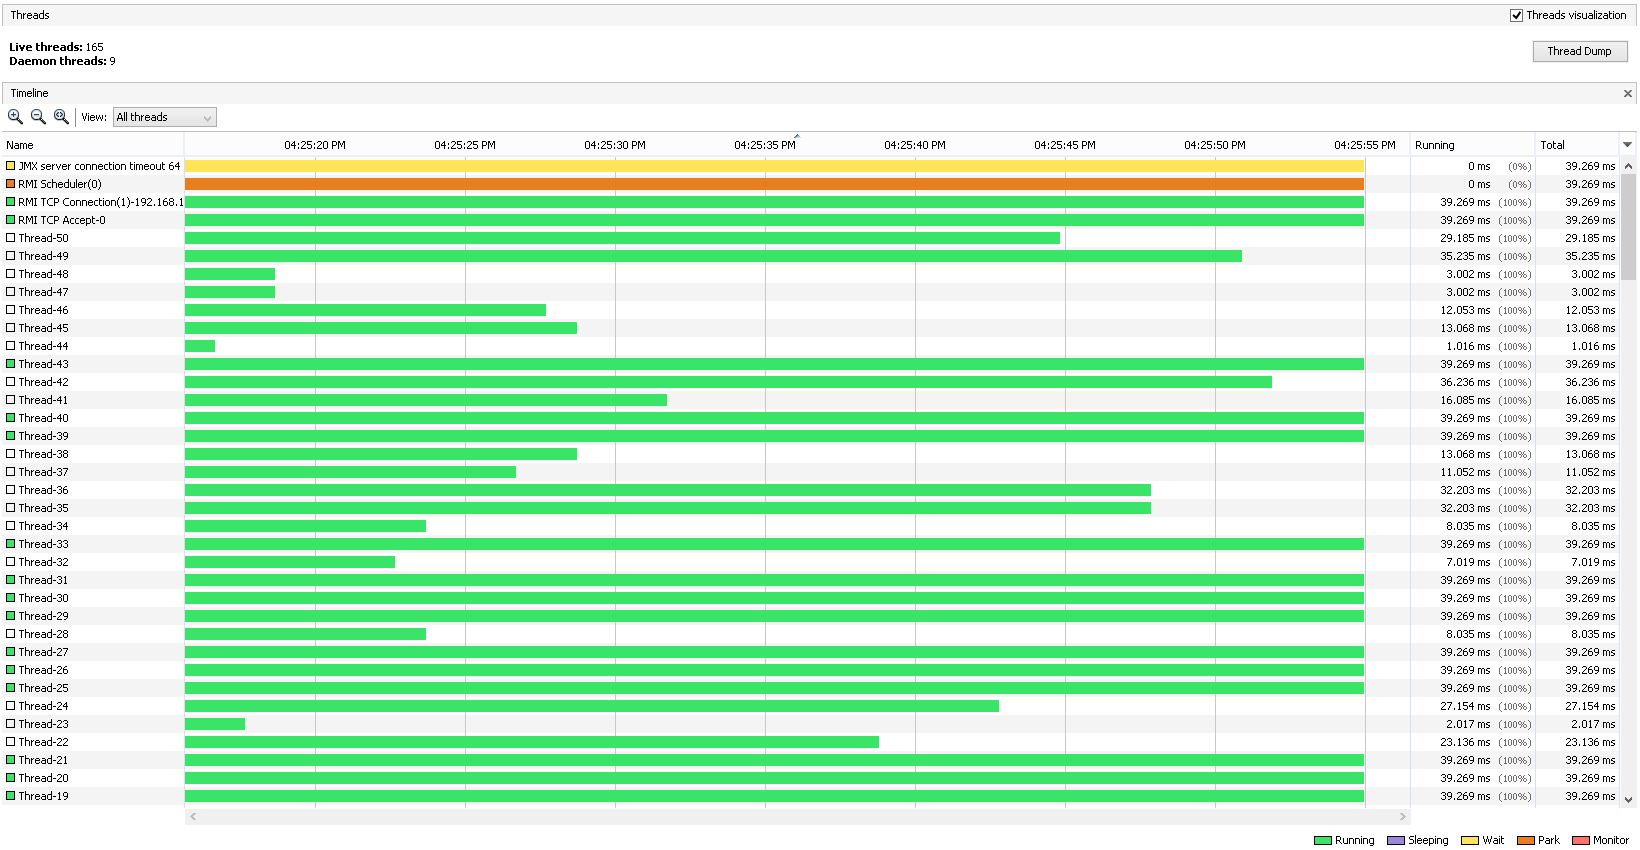
\includegraphics[width=0.95\textwidth]{images/Running_Time_50_Threads}
\caption{\emph{Thread timeline}, con 50 hilos}
\label{fig:6.37}
\end{figure}

\begin{figure}[H]
\centering
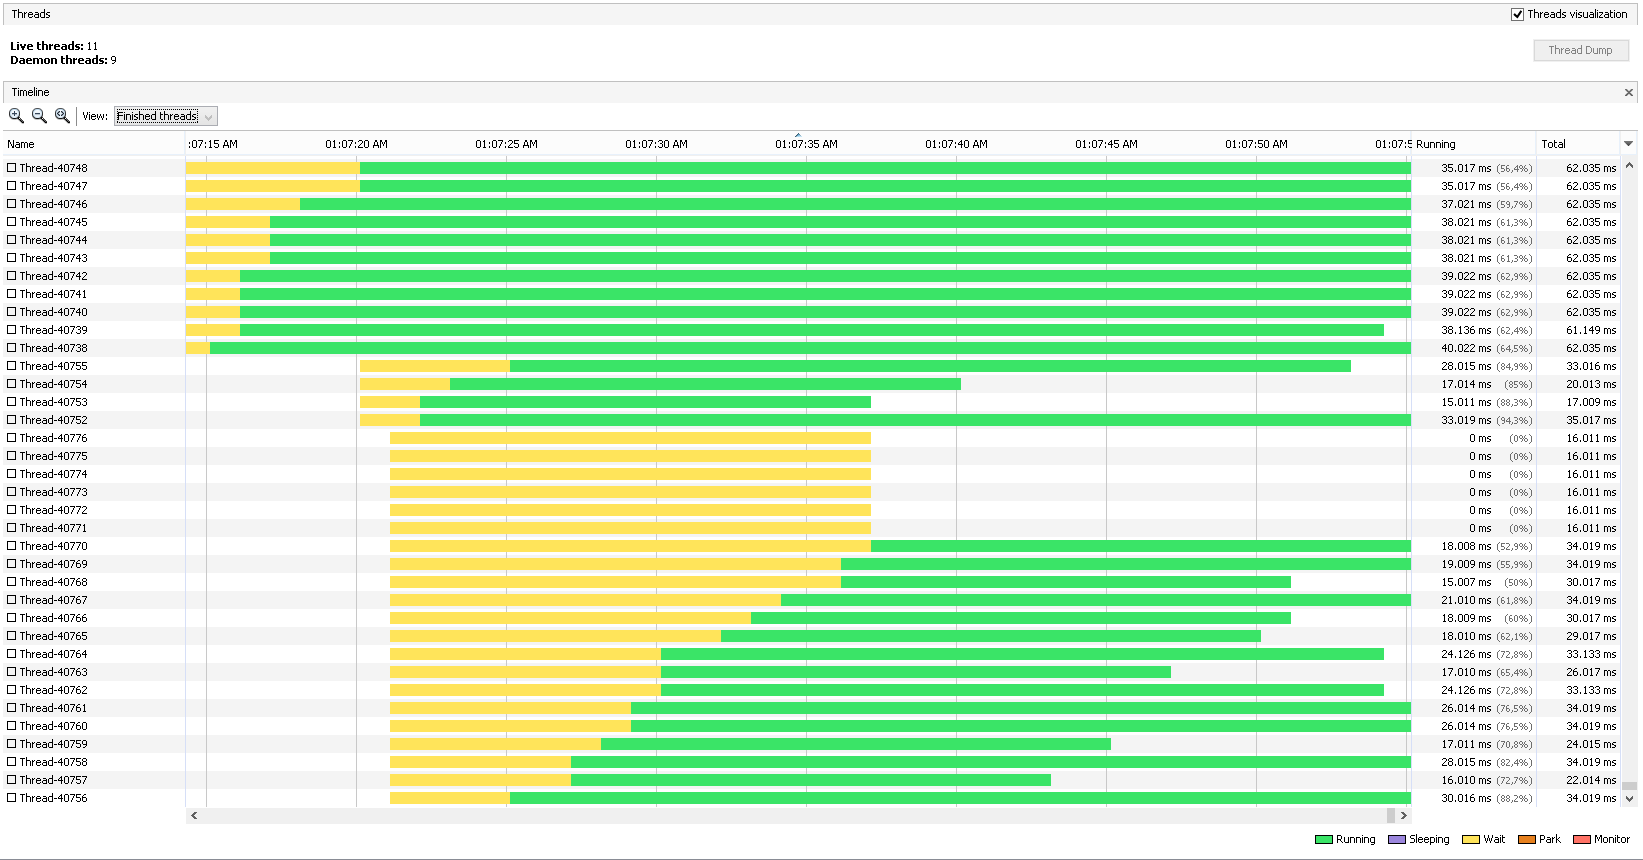
\includegraphics[width=0.95\textwidth]{images/Running_Time_50_Threads_Part_2}
\caption{\emph{Thread timeline}, segunda parte, con 50 hilos}
\label{fig:6.38}
\end{figure}

\begin{figure}[H]
\centering
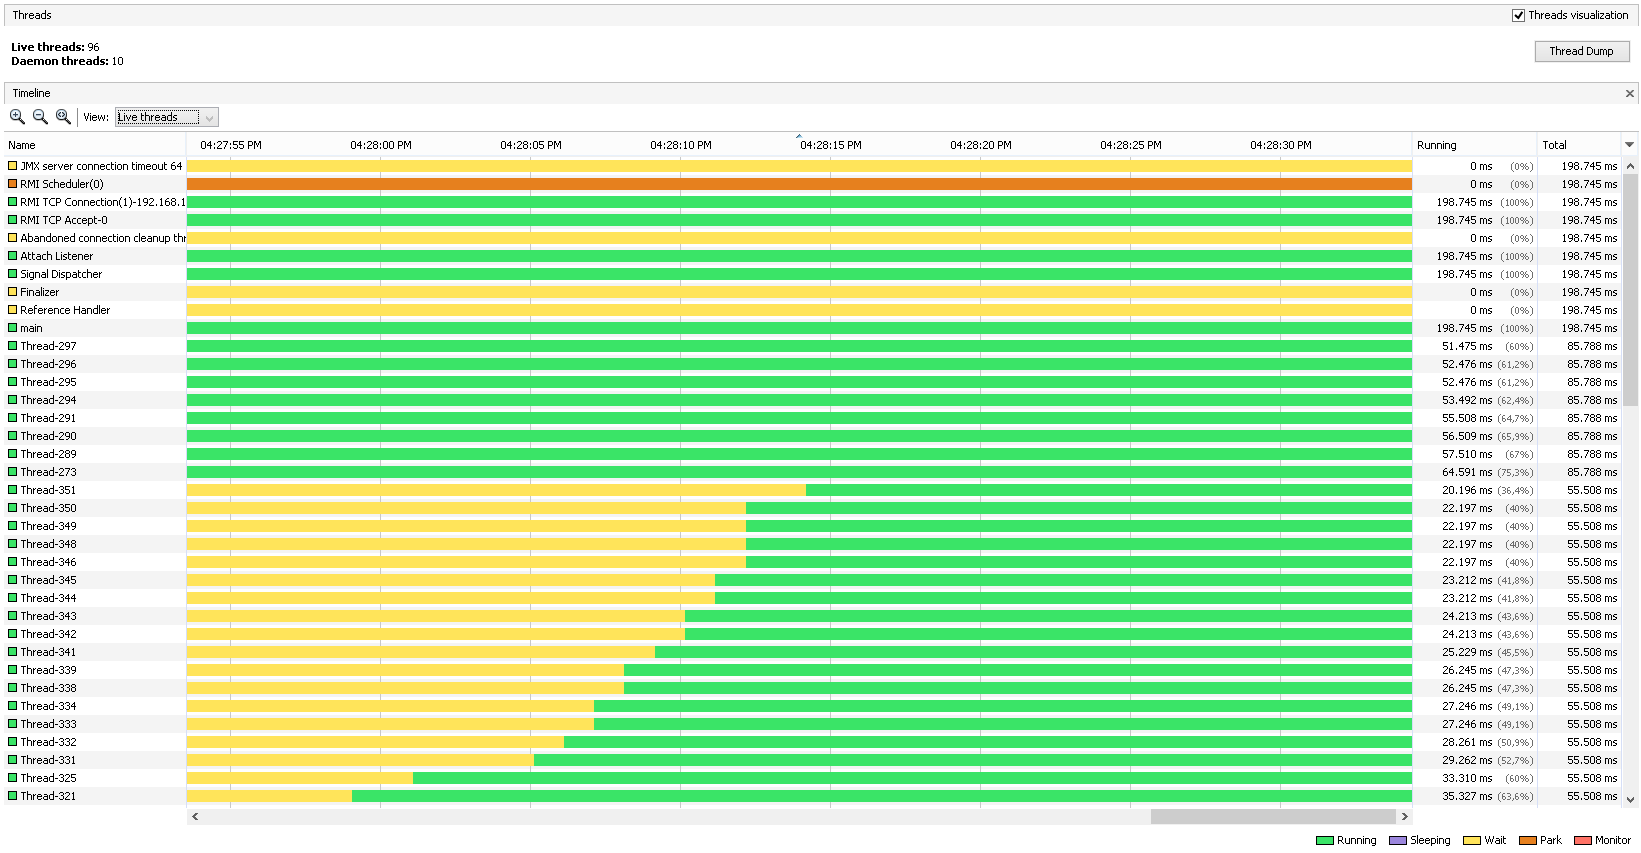
\includegraphics[width=0.95\textwidth]{images/Running_Time_50_Threads_Waits}
\caption{\emph{Thread timeline}, tercera parte, con 50 hilos}
\label{fig:6.39}
\end{figure}

\subsection{Resumen de las pruebas}
\noindent
En la presente secci'on se muestra una tabla resumen con los resultados arrojados de las diferentes pruebas.

\begin{table}[H]
\begin{center}
\scalebox{0.8}{	
\begin{tabular}{| l || c | c | c | c | c | c |}
\hline
\textbf{Prueba} & \textbf{Cantidad de hilos} & \textbf{Tiempo promedio} & \textbf{Total archivos} & \textbf{Total archivos} & \textbf{Aceleraci'on} \\ 
& & \textbf{de ejecuci'on} & \textbf{procesados} & \textbf{procesados} &\\ 
& & \textbf{(minutos)} & \textbf{con 'exito} & \textbf{con fallas} &\\ \hline \hline
Secuencial & 1 & 101.15 & 40775 & 0 & 1X \\ \hline
Paralelo & 8 & 48.34 & 40775 & 0  & 2.09X \\ 
Procesadores & & & & &\\ \hline
Paralelo & 10 & 46.27 & 40775 & 0 & 2.19X \\ 
Procesadores & & & & &\\ \hline
Paralelo & 16 & 67.06 & 40775 & 0 & 1.51X \\ 
Procesadores & & & & &\\ \hline
Paralelo & 32 & 474.58 & 40775 & 0 & 0.21X \\ 
Procesadores & & & & &\\ \hline
Paralelo & 50 & 522.86 & 40775 & 0 & 0.19X \\ 
Procesadores & & & & &\\ \hline
\end{tabular}}
\end{center}
\caption{Resumen: resultados de las pruebas}
\end{table}

Como se puede evidenciar en la tabla 6.11, el mejor tiempo de ejecuci'on y el mejor aprovechamiento de los recursos computacionales se logr'o con la prueba en paralelo con 10 hilos de ejecuci'on.\\

\subsection{Clustering}
\noindent
A continuaci'on se detallan los resultados de la prueba de \emph{clustering} para los valores tomados de los \emph{observation files} de aquellas 'epocas que tuvieran alg'un deslizamiento de ciclo en los tipos L1 y L2:\\

N'umero de instancias: 3,874,181\\
N'umero de iteraciones realizadas para construir el modelo: 28\\
Tiempo que tard'o en construirse el modelo: 227.85 segundos.\\

\begin{table}[H]
\begin{center}
\scalebox{0.9}{	
\begin{tabular}{| l || l | l | l | l | }
\hline
\textbf{Atributo} & \textbf{Cluster 1} & \textbf{Cluster 2} & \textbf{Cluster 3} & \textbf{Cluster 4} \\ \hline \hline
Epoch date & 2014-04-30 & 2014-04-30 & 2014-04-30 & 2014-04-30 \\ 
& 22:35:13 & 23:32:31 & 22:16:12 & 22:16:07 \\ \hline
Sat'elites disponibles & 19.03 & 15.67 & 18.17 & 15.76 \\ \hline
Sat'elites Glonass & 8.14 & 6.83 & 8.41 & 6.18 \\ \hline
Sat'elites GPS & 10.89 & 8.84 & 9.77 & 9.58 \\ \hline
Sat'elites SBAS & 0 & 0 & 0.0005 & 0 \\ \hline
Cantidad de deslizamientos & 55.62 & 59.55 & 18.94 & 21.38 \\ 
de ciclo en L1 y L2 & & & & \\ \hline
\end{tabular}}
\end{center}
\caption{Resultados \emph{clustering} centroides}
\end{table}

Es necesario aclarar que los valores expuestos hacen referencia a la media o promedio de los valores observados.\\

\begin{table}[H]
\begin{center}
\scalebox{0.9}{	
\begin{tabular}{| l || l | l |}
\hline
\textbf{Cluster} & \textbf{Cantidad de instancias} & \textbf{Porcentaje} \\ \hline \hline
1 & 821,240 & 21 \\ \hline
2 & 1,394,169 & 36 \\ \hline
3 & 758,616 & 20 \\ \hline
4 & 900,156 & 23 \\ \hline
\end{tabular}}
\end{center}
\caption{Resultados \emph{clustering} instancias}
\end{table}

En la presente tabla se exponen los resultados de la prueba de \emph{clustering}, en donde los datos se encuentran agrupados por d'ias.\\

N'umero de instancias: 134\\
N'umero de iteraciones realizadas para construir el modelo: 5\\
Tiempo que tard'o en construirse el modelo: 0.02 segundos.\\

\begin{table}[H]
\begin{center}
\scalebox{0.9}{	
\begin{tabular}{| l || l | l | l | l | }
\hline
\textbf{Atributo} & \textbf{Cluster 1} & \textbf{Cluster 2} & \textbf{Cluster 3} & \textbf{Cluster 4} \\ \hline \hline
Epoch date & 2014-05-08 & 2014-05-01 & 2014-05-21 & 2014-04-30 \\ \hline
Sat'elites disponibles & 9.83 & 17.73 & 18 & 16.35 \\ \hline
Sat'elites Glonass & 8.33 & 8.37 & 8.55 & 6.27 \\ \hline
Sat'elites GPS & 1.5 & 9.37 & 9.44 & 10.08 \\ \hline
Sat'elites SBAS & 0 & 0 & 0 & 0 \\ \hline
Cantidad de deslizamientos & 801,016.67 & 496,652.85 & 2,431,711.04 & 1,396,281.27 \\ 
de ciclo en L1 y L2 & & & & \\ \hline
\end{tabular}}
\end{center}
\caption{Resultados \emph{clustering} centroides agrupado por d'ias}
\end{table}

\begin{table}[H]
\begin{center}
\scalebox{0.9}{	
\begin{tabular}{| l || l | l |}
\hline
\textbf{Cluster} & \textbf{Cantidad de instancias} & \textbf{Porcentaje} \\ \hline \hline
1 & 6 & 4 \\ \hline
2 & 52 & 39 \\ \hline
3 & 27 & 20 \\ \hline
4 & 49 & 37 \\ \hline
\end{tabular}}
\end{center}
\caption{Resultados \emph{clustering} instancias agrupado por d'ias}
\end{table}

\section{An'alisis de los resultados}
\noindent
De acuerdo a lo presentado en la secci'on anterior se observ'o que el rendimiendo de la aplicaci'on no mejor'o al configurarle un gran n'umero de hilos, sino que por el contrario, su rendimiento cay'o a tal punto que es mejor ejecutar el programa de modo secuencial que de modo paralelo. Este resultado no fue algo tan esperado por la investigaci'on, dado que siempre se procuro por buscar el mejor rendimiento posible. \\

Sin embargo, se encontr'o mejor'ia al correr el programa con 8 o 10 hilos, lo cual aument'o el rendimiento casi el triple de veces. Esto se debe a que a los programas paralelos dependen de encontrar el mejor balance entre el hardware disponible y el compilador. Se evidenci'o que entre m'as se sobrepasaba la capacidad de \emph{cores} del \emph{workstation}, mayor era el tiempo que tomaba en ejecutar la aplicaci'on, al crear colas de procesos para la asignaci'on d'inamica de recursos y se creaba mayor \emph{overhead} en la comunicaci'on entre los \emph{threads}. \\

Como era de esperarse, el \emph{Perm Space} se mantuvo sin mayores cambios a lo largo de las diferentes pruebas, con algunos picos (25 MB) cuando se optimiza el hardware del \emph{workstation}, es decir, cuando se hace un uso efectivo de los multiprocesadores.\\

Por el contrario, el \emph{Heap Space} tuvo diferentes cambios a lo largo de las pruebas. En el modo serial se comport'o casi de manera constante con un uso aproximadamente de unos 128MB. En el modo paralelo con 8 y 10 \emph{Threads} obtuvo un pico al comienzo de la ejecuci'on de un poco m'as de 1000MB, esto debido a la primera asignaci'on de recursos por parte del Sistema Operativo, mientras se distribu'ia entre los \emph{cores}. Luego al distribuir de manera eficiente la carga se visualiza un promedio de unos 450MB, con ciertos picos hasta casi los 700MB debido a los diferentes tama'nos de los archivos.\\

Con el uso 16 \emph{Threads} result'o en un gasto considerable de memoria, pues en 3/4 de la ejecuci'on se mantuvo un alto consumo de espacio, el promedio fue de aproximadamente los 1000MB. Esto quiere decir que la cola de procesos obtuvo una r'apida asignaci'on de recursos por parte del sistema operativo y se mantuvo con muchos objetos en memoria dado que la recuperaci'on de memoria fue m'as lenta que la instanciaci'on de objetos de la aplicaci'on. \\

En cuanto a las pruebas con m'as de 16 \emph{Threads}, se obtuvieron valores constantes, alrededor de los 90MB en el \emph{Heap Space}, lo cual lo interpretamos de que la cola de procesos era muy grande y por lo cual el sistema operativo distribuy'o las cargas de trabajo sin mayor prioridad entre los diferentes \emph{cores}, lo cual hizo que estos valores no cambiaran a lo largo de la ejecuci'on y se presentara un rendimiento menor que en el modo secuencial.\\

Se puede evidenciar f'acilmente a trav'es de los gr'aficos de ``vida'' de los \emph{Threads} el tiempo promedio y de la cantidad de hilos activos en cierto per'iodo de ejecuci'on, y en el cual se comprueba una gran cantidad de hilos activos al realizarce un mayor paralelismo en el ambiente de pruebas.\\

Para detallar un poco la diferencia entre el \emph{Heap Space} y el \emph{Perm Space} es que el primero almacena los datos de los objetos instanciados mientras que el segundo guarda las definiciones de las clases cargadas en la \emph{JVM}. Tambi'en es importante que el ciclo de vida del \emph{Heap Space} est'e ligado con la aplicaci'on y que el \emph{Perm Space} est'e ligado con la \emph{JVM}.\\

Por 'ultimo, haciendo referencia a las pruebas de \emph{clustering}, no fueron concluyentes los resultados con los datos colocados a la herramienta Weka. No se puede dar ning'un resultado relevante porque los grupos contaron con informaci'on muy similar y no hubo una clara evidencia de diferenciaci'on entre ellos.\\

\clearpage